\documentclass[11pt]{article}

% Packages
\usepackage{graphicx}   % for pictures
\usepackage{amsthm}     % for math
\usepackage{amsmath, mathtools}    %   more math
\usepackage{amsfonts}   %   more math
\usepackage{physics}    % more symbols
\usepackage{circuitikz} % for circuit diagrams
\usepackage{amssymb}    % math symbols
\usepackage{siunitx}    % units
\usepackage{mathrsfs}   % fancy text
\usepackage{color}      % colored letters for notes and reminders
\usepackage{float}      % for image location

%The amsthm package lets you format different types of mathematical ideas nicely. You use it by defining "\newtheorem"s as below:
\newtheorem{problem}{Problem}
\newtheorem{theorem}{Theorem}
\newtheorem*{proposition}{Proposition}
\newtheorem{lemma}[theorem]{Lemma}
\newtheorem{corollary}[theorem]{Corollary}
\theoremstyle{definition}
\newtheorem{defn}[theorem]{Definition}

% Magins

\setlength{\voffset}{0.1in}
\setlength{\paperwidth}{8.5in}
\setlength{\paperheight}{11in}
\setlength{\headheight}{14pt}
\setlength{\headsep}{0.5in}
\setlength{\textheight}{11in}
\setlength{\textheight}{8in}
\setlength{\topmargin}{-0.25in}
\setlength{\textwidth}{7in}
\setlength{\topskip}{0in}
\setlength{\oddsidemargin}{-0.25in}
\setlength{\evensidemargin}{-0.25in}

% For images in this document:
\graphicspath{ {images/} }

% User Defined Commands
\newcommand{\nder}[2]{\frac{d^{#1} #2}{d t^{#1}}}   % The nth derivative wrt t: {n}{x(t)}
\newcommand{\der}[1]{\frac{d #1}{d t}}              % Derivative wrt t: {x(t)}
\newcommand{\infint}{\int_{-\infty}^{\infty}}       % Integral from - infinity to + infinity
\newcommand{\infsum}[1]{\sum_{#1 = -\infty}^{\infty}}% Sum of a variable from - to + infinity
\newcommand{\para}[1]{\left( #1 \right)}            % Instead of writing parenthesis all the time

% User Command for Wider Matrices
\makeatletter
\renewcommand*\env@matrix[1][\arraystretch]{%
  \edef\arraystretch{#1}%
  \hskip -\arraycolsep
  \let\@ifnextchar\new@ifnextchar
  \array{*\c@MaxMatrixCols c}}
\makeatother


% Heading:
\usepackage{fancyhdr}
\pagestyle{fancy}
\lhead{Nicholas Pham}
\chead{ES 155}          %   Change the Class!!
\rhead{Homework 7}   %   Change the Problem Set Number!!


% ----- BEGIN DOCUMENT-----
\begin{document}

\textbf{\huge{ES 155 Homework 7}}    %   Change the Class and Problem Set Number!!
\normalsize

\begin{enumerate}
    \item % Problem 1
    When deriving the transfer function $G_{a\rightarrow b}$, assume all other inputs (besides $a$ and $b$) are 0.

    \begin{enumerate}
        \item        
        \begin{align*}
            G_{r \rightarrow e} &= \frac{E(s)}{R(s)} \\
            E(s) &= R(s) - H(s)\\ 
            &= R(s) - P(s)C(s)E(s) \\
            &= \frac{1}{1 + P(s)C(s)} R(s) \\
            G_{r \rightarrow e} &= \frac{1}{1 + P(s)C(s)}
        \end{align*}

        \item        
        \begin{align*}
            G_{d \rightarrow e} &= \frac{E(s)}{D(s)} \\
            E(s) &= -Y(s) = -P(s) \big( D(s) + C(s)E(s) \big) \\
            &= \frac{P(s)C(s)}{1 + P(s)C(s)} D(s) \\
            G_{d \rightarrow e} &= \frac{P(s)C(s)}{1 + P(s)C(s)}
        \end{align*}

        \item        
        \begin{align*}
            G_{n \rightarrow e} &= \frac{E(s)}{N(s)} \\
            E(s) &= -Y(s) = -\big( N(s) + P(s)C(s)E(s) \big) \\
            &= \frac{-N(s)}{1 + P(s)C(s)} \\
            G_{n \rightarrow e} &= - \frac{1}{1 + P(s)C(s)}
        \end{align*}        

        \item        
        \begin{align*}
            G_{r \rightarrow y} &= \frac{Y(s)}{R(s)} \\
            Y(s) &= P(s)C(s)E(s) = P(s)C(s) \big( R(s) - Y(s) \big) \\
            &= \frac{P(s)C(s)}{1 + P(s)C(s)}R(s) \\
            G_{r \rightarrow y} &= \frac{P(s)C(s)}{1 + P(s)C(s)}
        \end{align*}   

        \item
        \begin{align*}
            G_{d \rightarrow y} &= \frac{Y(s)}{D(s)} \\
            Y(s) &= P(s) \big( D(s) + C(s)E(s) \big) \\
            &= P(s) \big( D(s) - C(s)Y(s) \big) \\
            &= \frac{P(s)}{1 + P(s)C(s)} D(s) \\
            G_{d \rightarrow y} &= \frac{P(s)}{1 + P(s)C(s)}
        \end{align*} 

        \item
        \begin{align*}
            G_{n \rightarrow y} &= \frac{Y(s)}{N(s)} \\
            Y(s) &= N(s) + P(s)C(s)(-Y(s)) \\
            Y(s) &= \frac{1}{1 + P(s)C(s)}N(s) \\
            G_{n \rightarrow y} &= \frac{1}{1 + P(s)C(s)}
        \end{align*} 
    \end{enumerate}
    \item % Problem 2
        \begin{enumerate}
            \item % 2.a
            $$ G_1(s) = \frac{1}{(s + a)(s + 10a)} $$
            \begin{figure}[H]
                \centering
                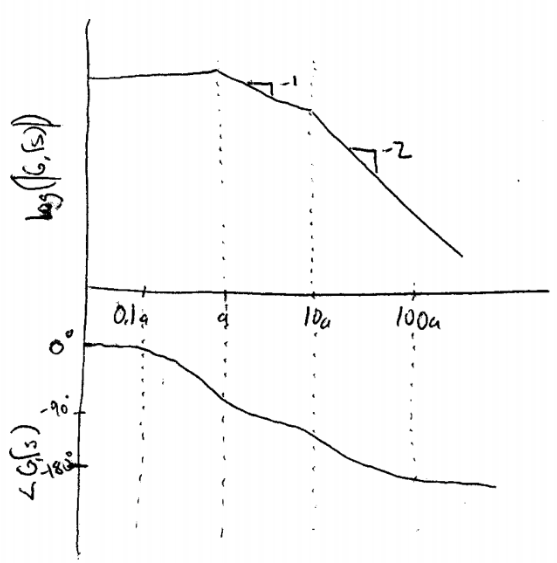
\includegraphics[width = 0.5\textwidth]{ES155P7_2a}
            \end{figure}
            \item % 2.b
            $$ G_2(s) = \frac{1 + s/a}{s + 10a} = \left(\frac{1}{a}\right)\frac{s + a}{s + 10a} $$
            The DC gain is $20\log \frac{1}{10 a}$.
            \begin{figure}[H]
                \centering
                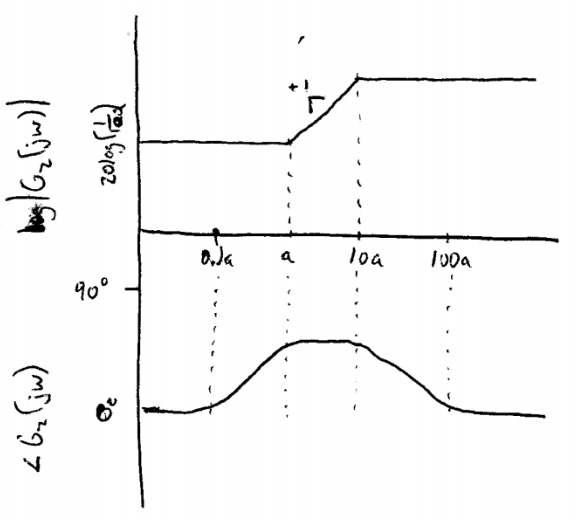
\includegraphics[width = 0.5\textwidth]{ES155P7_2b}
            \end{figure}
            \item % 2.c
            $$ G_3(s) = \frac{s + a}{s + 2a} $$
            \begin{figure}[H]
                \centering
                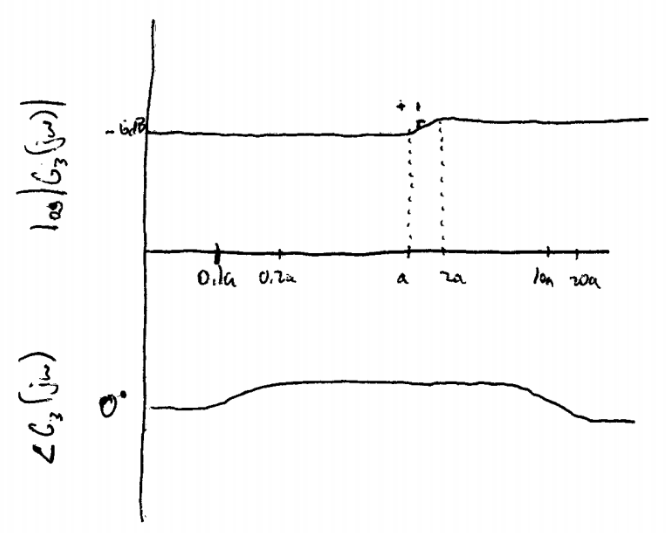
\includegraphics[width = 0.5\textwidth]{ES155P7_2c}
            \end{figure}
            \item % 2.d
            $$ G_4(s) = \frac{1}{s^2 + 2 \zeta \omega s + \omega ^2} $$
            \begin{figure}[H]
                \centering
                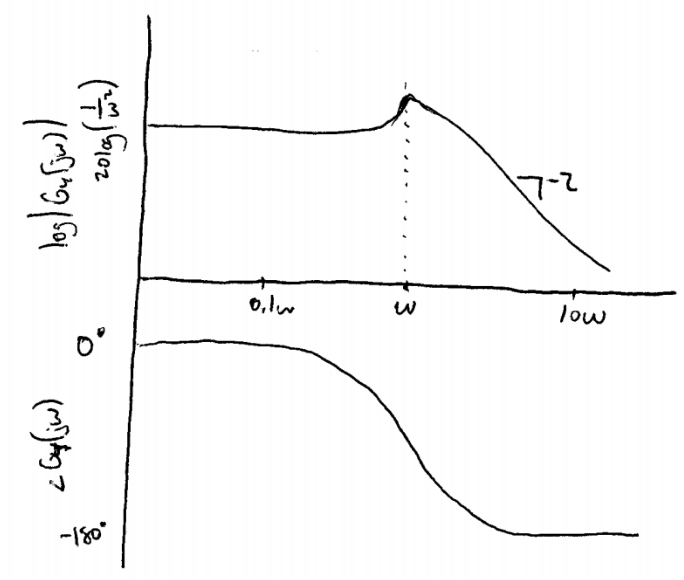
\includegraphics[width = 0.5\textwidth]{ES155P7_2d}
            \end{figure}
        \end{enumerate}

    \item % Problem 3
    The open loop transfer function is $L(s) = P(s) C(s)$.  This transfer function can be used directly in MATLAB to plot the Bode and Nyquist plots.  See attached MATLAB code for the Bode and Nyquist plots, as well as the computation of the gain and phase margins.  Figure \ref{fig:3a} shows the Bode and Nyquist plots from MATLAB for the disk drive transfer function $P(s)C(s)$ where

    $$ P(s) = \frac{1}{s^3 + 10s^2 + 3s + 10} \quad \text{and} \quad C(s) = 1000 \frac{s+1}{s+10} $$

    \begin{figure}[H]
        \centering
        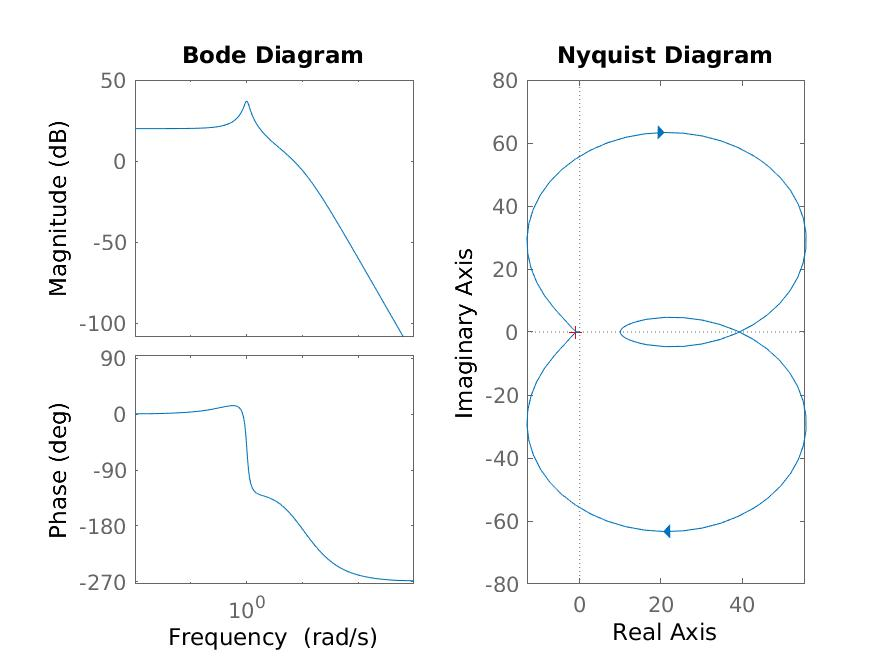
\includegraphics[width = 0.8\textwidth]{ES155P7_3a.jpg}
        \caption{Disk drive transfer function.  The gain margin is 1.6047 and the phase margin is 12.9616.}
        \label{fig:3a}
    \end{figure}

    Figure \ref{fig:3b} shows the Bode and Nyquist plots from MATLAB for the second order PD transfer function $P(s)C(s)$ where

    $$ P(s) = \frac{100}{(100s + 1)(s + 1)} \quad \text{and} \quad C = s + 10 $$

    \begin{figure}[H]
        \centering
        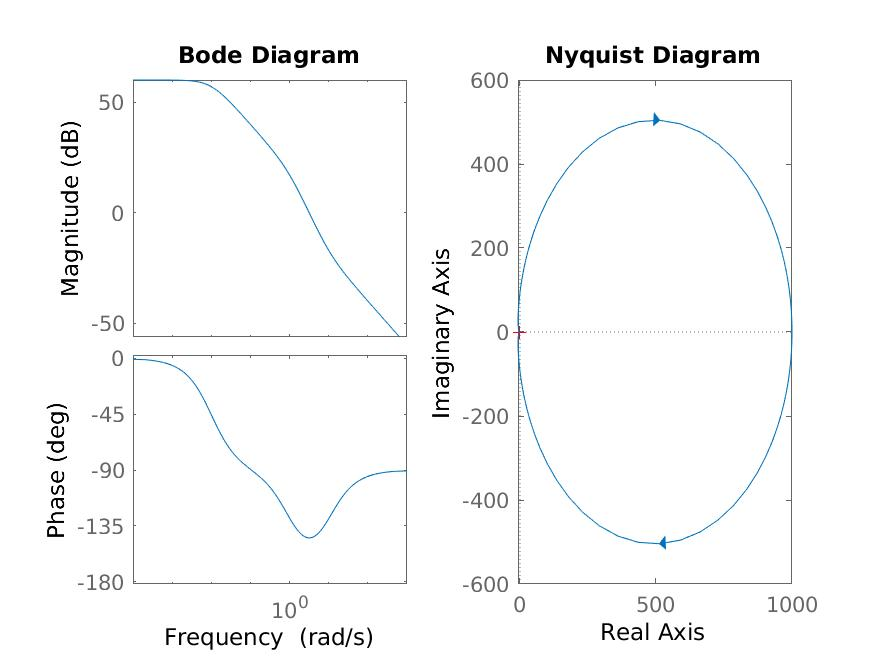
\includegraphics[width = 0.8\textwidth]{ES155P7_3b.jpg}
        \caption{PD transfer function.  The gain margin reported by MATLAB is $\infty$ while the phase margin is 35.2780.  This might not be an error, as the system has two poles and one zero, which means the phase at high frequencies is -90dB.}
        \label{fig:3b}
    \end{figure}


    \item % Problem 4
    The dynamics for the system are

    $$ P(s) = \frac{Tba/m}{(s+a)(s+c/m)} = \frac{Tba}{(s + a)(ms + c)} = \frac{Tba}{ms^2 + (am + c)s + ac} $$

    This plant transfer function is modelled in MATLAB.

    \begin{enumerate}
        \item % 4.a
        The proportional integral controller

        $$C(s) = k_p + \frac{k_i}{s} = \frac{k_p s + k_i}{s} $$

        can also be modelled in MATLAB.  The phase and gain margins, rise time, and overshoot are computed via $\mathtt{stepinfo()}$ and plotted in the table.

        \begin{center}
        \begin{tabular}{|c c|c c c c c c|}
        \hline
        $k_p$ & $k_i$ & Stable & $g_m$ & $\varphi_m$ & SS$_{err}$ & $T_r$ & $M_p$ \\
        \hline
            0.5000 &   0.1000 &   1 &      $\infty$ &      118.1865 &   0.0950 &  24.2034 &        0 \\
            0.0500 &   1.0000 &   1 &      $\infty$ &       54.7945 &   0.0070 &   1.6819 &  14.2429 \\
            0.0500 &   0.0010 &   1 &      $\infty$ &      $\infty$ &   0.9095 & 149.6098 &        0 \\
            0.0050 &   0.0010 &   1 &      $\infty$ &      $\infty$ &   0.9091 & 200.4907 &        0 \\
        \hline
        \end{tabular}
        \end{center}

        \item % 4.b
        Figure \ref{fig:4bplots} shows the zero-pole diagrams and step responses for the closed loop systems.  

        \begin{figure}[H]
            \centering
            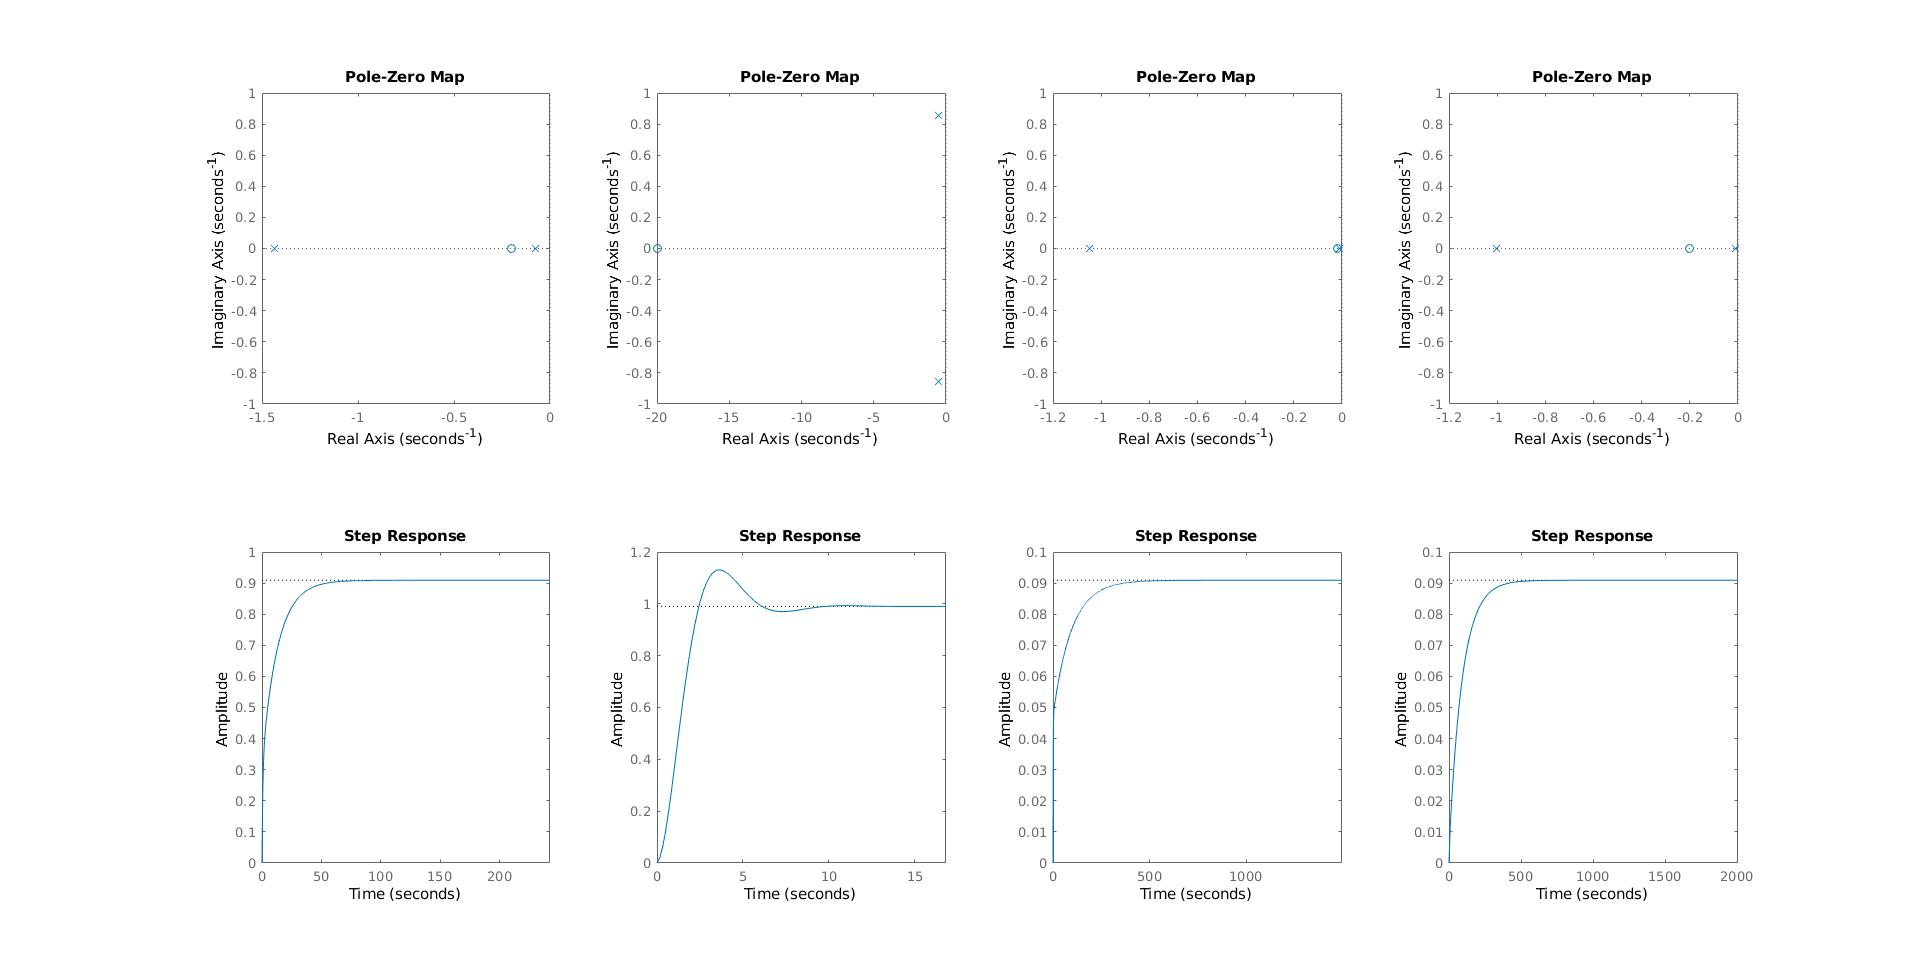
\includegraphics[width = \textwidth]{ES155P7_4b_plots.jpg}
            \caption{Top: Pole-Zero diagrams.  Bottom: Step Responses.  From left to right, the $k_p$ and $k_i$ parameters are (0.5, 0.1), (0.05, 1), (0.05, 0.001), and (0.005, 0.001).}
            \label{fig:4bplots}
        \end{figure}

        \item % 4.c

        The table shows that all of the closed loop systems are stable, as evidenced by the Nyquist plots in Figure \ref{fig:4b_bodenyquist}, shows the corresponding Bode and Nyquist plots for the same closed loop systems.  None of the plots encircles (-1,0), so the systems are stable.  This is reflected in the step responses shown in Figure \ref{fig:4bplots}.  Their gain margins are all $\infty$, as any amount of gain applied will never result in the Nyquist plot encircling (-1, 0), as none of them cross the real axis left of the origin.  The error was relatively low for the first and second systems, which had relatively stronger parameters than the latter ones.  Once the controllers' strength decreased too much, they were unable to correct the system, and it sat around 1/10 the desired value.  For these later systems, the rise time was very long as well, because of these weak controls.  The second system had a very strong integral term which resulted in a damped oscillatory response, allowing it to have a much shorter rise time than the first system.  However, this also resulted in overshoot, which none of the other systems exhibit.

        \begin{figure}[H]
            \centering
            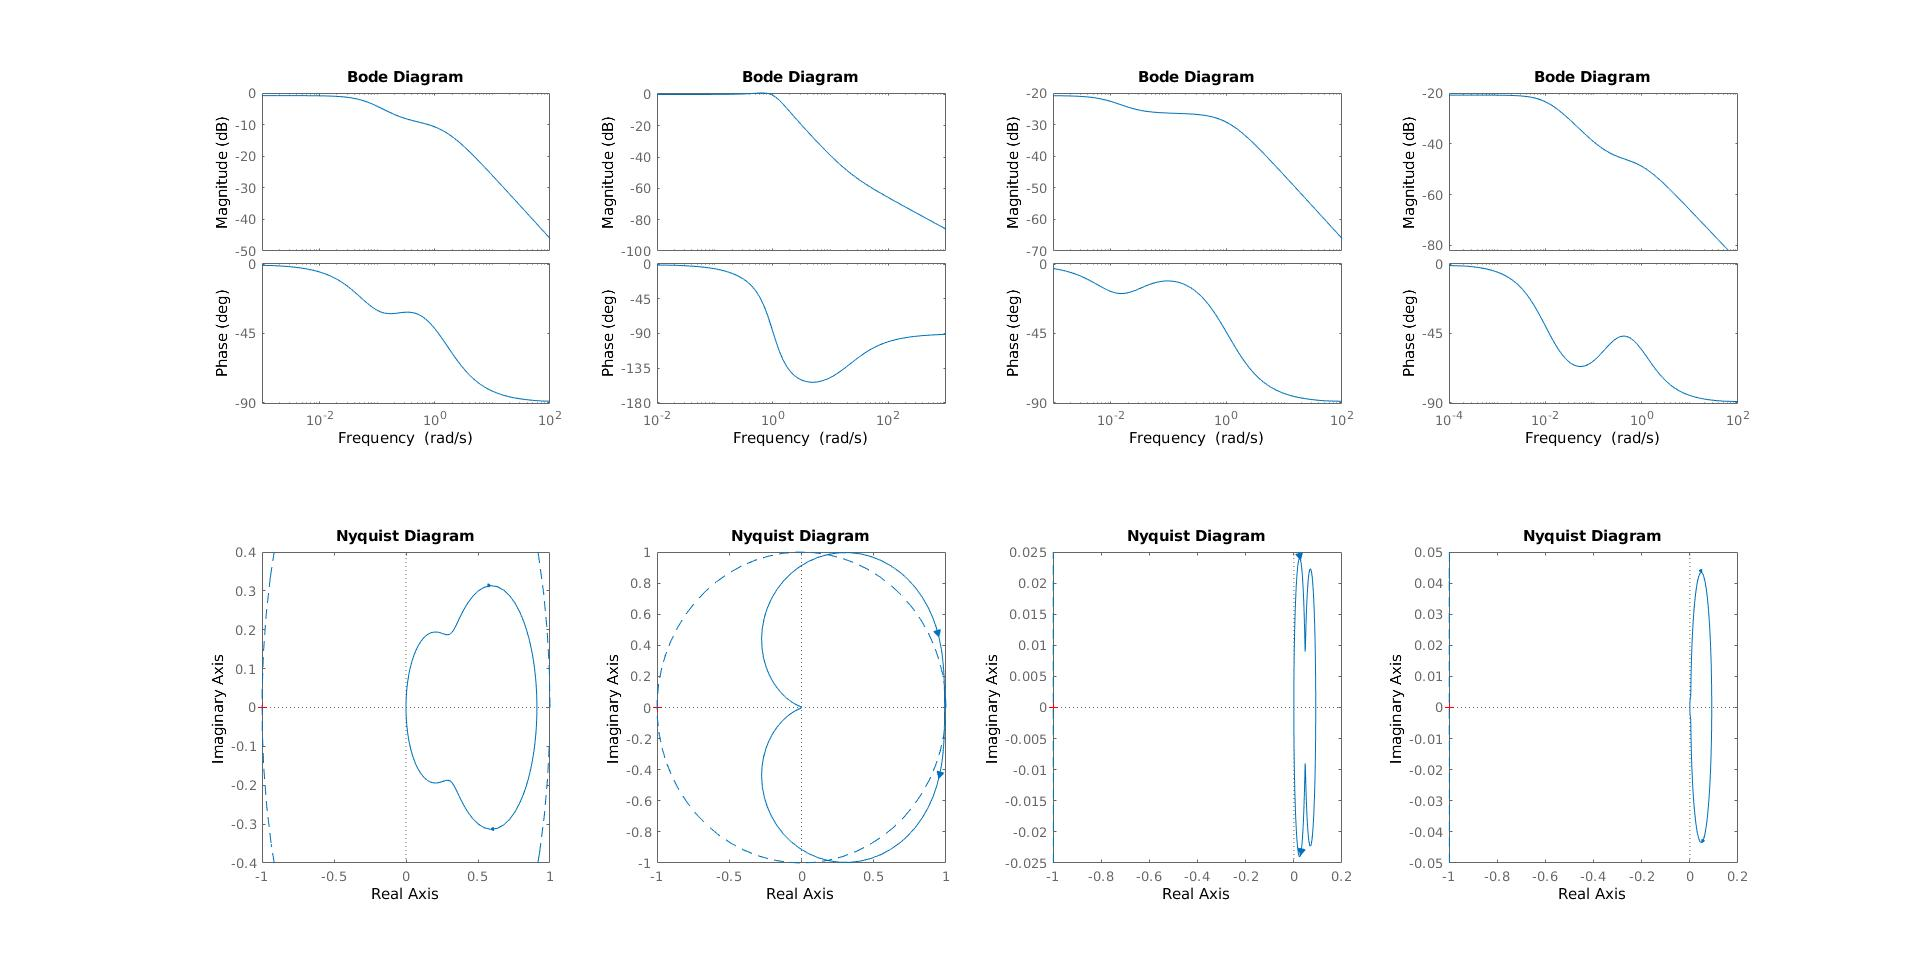
\includegraphics[width = \textwidth]{ES155P7_4b_bodenyquist.jpg}
            \caption{Top: Bode diagrams.  Bottom: Nyquist plots.  From left to right, the $k_p$ and $k_i$ parameters are (0.5, 0.1), (0.05, 1), (0.05, 0.001), and (0.005, 0.001).}
            \label{fig:4b_bodenyquist}
        \end{figure}

    \end{enumerate}

\end{enumerate}
\end{document}


